% --- Books ---
% - https://www.amazon.de/Docker-Software-entwickeln-deployen-Containern/dp/386490384X/ref=sr_1_1?ie=UTF8&qid=1483784437&sr=8-1&keywords=docker
% - https://www.amazon.com/Docker-Action-Jeff-Nickoloff/dp/1633430235/ref=sr_1_1?ie=UTF8&qid=1483784469&sr=8-1&keywords=docker
% - https://www.amazon.com/Docker-Practice-Ian-Miell/dp/1617292729/ref=sr_1_10?ie=UTF8&qid=1483784469&sr=8-10&keywords=docker
% - https://www.amazon.com/Developing-Docker-Jaroslaw-Krochmalski-ebook/dp/B01GEJKJ6A/ref=sr_1_33?ie=UTF8&qid=1483784510&sr=8-33&keywords=docker

\chapter{Docker}
\label{cha:docker}
Wie in \cref{sec:vollvirtualisierung} beschrieben, ermöglicht die Virtualisierung von IT-Systemen eine Abstraktion der Hardware.
Ressourcen lassen sich effizienter nutzen, die Systeme werden jedoch nicht optimal ausgenützt, da das gesamte Betriebssystem virtualisiert wird.
Dies führt zu langen Startzeiten und einem hohen Speicherverbrauch.

Containervirtualisierung (siehe \cref{sec:containervirtualisierung}) löst diese Probleme durch die Wiederverwendung des Kernels.
Dadurch entsteht die Möglichkeit, Anwendungen mitsamt den benötigten Systemressourcen zu verpacken und die Abhängigkeiten für den Betrieb zu reduzieren.
Für einen Container wird lediglich die Laufzeitumgebung benötigt, ist diese installiert, ist garantiert, dass der Container funktioniert.
Docker\footnote{\url{https://www.docker.com/}} wird in 94\% (Stand Juni 2016) der Unternehmen eingesetzt, die auf Containervirtualisierung setzen \autocite{ContainerAdoption}.

\section{Geschichte}
\label{sec:docker-history}
Der Blogeintrag \autocite{redhat-container-history:online} schildert die Geschichte der Containervirtualisierung.

Im Jahr 2001 ermöglicht Jacques Gélinas mithilfe eines gepatchten Kernels zum ersten Mal das Ausführen mehrerer Linux-Server auf einem einzelnen Rechner, ohne auf Vollvirtualisierung zurückzugreifen.

2006 folgt die Aufnahme von cgroups in den Linux-Kernel, worauf 2008 die Implementierung der namespaces folgt.
Ebenfalls 2008 beginnt IBM mit der Entwicklung von LXC, wobei auf cgroups und namespaces aufgesetzt wird.
% http://searchservervirtualization.techtarget.com/feature/A-brief-history-of-Docker-Containers-overnight-success
% http://blog.aquasec.com/a-brief-history-of-containers-from-1970s-chroot-to-docker-2016

2013 wird Docker als Open-Source-Projekt der Platform-as-a-Service-Umgebung dotCloud vorgestellt.
Docker führt nichts wesentlich Neues ein, sondern bietet lediglich für die bestehenden Technologien wie LXC eine sehr einfach zu verwendende Benutzerschnittstelle, die Container für eine breite Benutzergruppe zugänglich macht.

2014 erscheint Docker in der Version 1.0, nachdem mit Version 0.9 LXC als Containerumgebung durch \emph{libcontainer\footnote{\url{https://github.com/opencontainers/runc/tree/master/libcontainer}}} ersetzt wird.
libcontainer ist eine Eigenentwicklung von Docker, die in der Programmiersprache Go geschrieben ist und die Verwaltung und Ausführung von Containern ermöglicht.

2015 tritt Docker der Open Container Initiative bei, wodurch die Quelltexte und Entwicklungen dem unter der Linux Foundation stehenden Projekt hinzugefügt werden.
Dieser Schritt verstummt Kritiker, die eine Monopolstellung von Docker befürchtet haben.
Seit 2015 werden hauptsächlich Fehlerbehebungen und Verbesserungen an Docker selbst durchgeführt, sowie das Docker-Ökosystem durch zahlreiche Werkzeuge erweitert (siehe \cref{sec:docker-products}).

Die in diesem Kapitel gezeigten Beispiele und verwendeten Funktionen basieren auf der Docker-Version 1.13 vom 19. Jänner 2017.
\section{Funktionsweise}
\label{sec:docker-basics}
Die Funktionsweise von Docker wird in \autocite{docker-overview:online} beschrieben und im folgenden Abschnitt zusammengefasst.
Docker basiert auf einer Vielzahl von Komponenten, die erst als Gesamtsystem eine Containervirtualisierung ermöglichen.
Ein grundlegendes Wissen über diese Komponenten ist für die Verwendung von Docker unerlässlich.
\begin{description}
    \item [daemon] Im Hintergrund von Docker läuft der Server-Prozess, genannt \texttt{daemon}, der sich um das Anlegen und Verwalten von \texttt{images}, \texttt{containern}, \texttt{networks} und \texttt{data volumes} kümmert.
    Er läuft auf dem Host-System und nimmt Kommandos der \texttt{clients} über eine REST-Schnittstelle entgegen.
    \item [client] Der \texttt{client} ist die Benutzeroberfläche von Docker, die in Form einer Kommandozeilenanwendung zur Verfügung steht.
    Er nimmt Kommandos und Konfigurationen entgegen und sendet diese an einen zuvor festgelegten \texttt{daemon}.
    \item [engine] Als \texttt{engine} wird die Kombination aus \texttt{daemon} und \texttt{client} bezeichnet, die den Kern von Docker bildet.
    \item [image] Ein \texttt{image} ist eine Vorlage für das Erstellen eines \texttt{containers}. \texttt{Images} können erweitert und dadurch wiederverwendet werden und bilden die Basis zum Erstellen eines \texttt{containers}. Images sollten immer deklarativ mihilfe von Dockerfiles (siehe \cref{sec:dockerfiles}) erstellt werden.
    \item [container] \texttt{Container} sind jene Teile, die von Docker ausgeführt werden. Sie sind die ausführbare Instanz eines \texttt{images}. \texttt{Container} werden vom \texttt{daemon} gestartet, gestoppt, verschoben oder gelöscht, der die Anweisungen vom \texttt{client} enthält. Zusätzlich können \texttt{container} zur Inter-Container-Kommunikation Netzwerken zugewiesen werden, oder zur Datenpersistierung mit Speicherbereichen versorgt werden.
    \item [registry] \texttt{Registrys} dienen der Verteilung von \texttt{images}. Sie stellen eine Bibliothek dieser dar und können entweder privat oder öffentlich zugänglich sein (siehe \cref{sec:docker-hub}).
    \item [service] Ein \texttt{service} ist eine Sammlung von Docker-Containern, welche durch einen Schwarmmanger (siehe \cref{sec:docker-swarm}) verwaltet wird und die Basis für Multi-Container-Anwendungen darstellt. Seit Docker 1.12 werden \texttt{services} in vollem Ausmaß unterstützt.
\end{description}
In \cref{lst:docker-run-basics} wird ein neuer Container auf Basis des Ubuntu-Images gestartet, in dem die Bash gestarte wird.
\begin{lstlisting}[caption=Ubuntu-Bash in Docker, language=bash, label=lst:docker-run-basics]
    $ docker run -i -t ubuntu /bin/bash
\end{lstlisting}
Dabei erledigt die Docker-Engine folgende Schritte:
\begin{enumerate}
    \item Das \texttt{ubuntu}-Docker-Image wird von der Docker-Registry heruntergeladen, falls dieses lokal noch nicht existiert.
    \item Ein neuer Container wird auf Basis des Images erstellt und mit einem zufälligen Namen versehen.
    \item Ein schreibfähiges Dateisystem wird zu dem eben erstellten Container hinzugefügt.
    \item Für den Container wird eine Netzwerkverbindung geschaffen, die eine Kommunikation mit dem Host ermöglicht. Standardmäßig wird die \texttt{bridged}-Schnittstelle verwendet.
    \item Der Container erhält eine IP-Adresse.
    \item Das angegebene Programm wird ausgeführt. In diesem Fall ist das \texttt{/bin/bash}.
    \item Die Parameter \texttt{-t} und \texttt{-i} führen dazu, dass die Standardeingabe und Standardausgabe verbunden werden und der Container in einen interaktiven Modus geschaltet wird. Der Benutzer befindet sich nun in der Bash in Ubuntu in Docker.
\end{enumerate}
In \cref{fig:docker-architektur} ist dieser Ablauf grafisch dargestellt.
\begin{figure}[htbp]
    \centering
    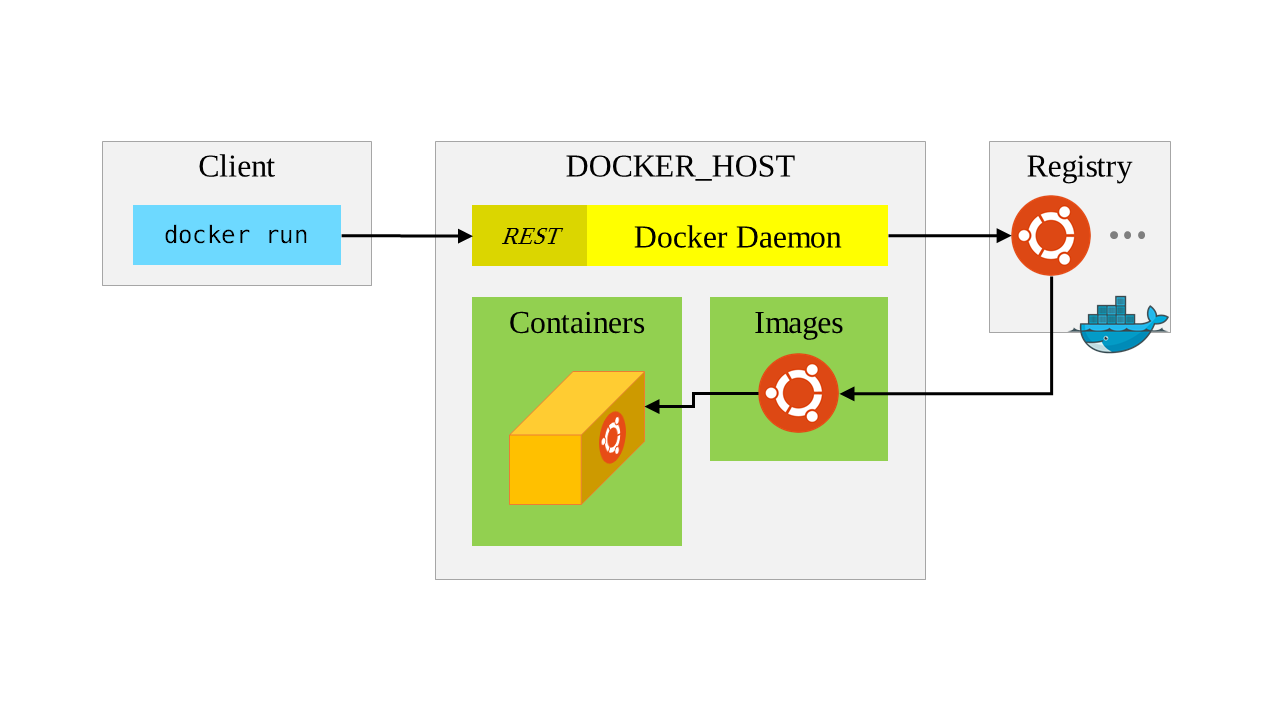
\includegraphics[width=0.9\linewidth,clip]{images/docker-architecture}
    \caption{Docker-Architektur}
\label{fig:docker-architektur}
\end{figure}


\section{Plattformen}
\label{sec:docker-platforms}
Docker läuft nur auf Linux-Versionen nativ, deren Kernels zu Docker kompatibel sind.
Auf allen anderen Systemen wird durch virtualisierte Umgebungen eine Möglichkeit geschaffen Docker auszuführen.
Bei diesen Werkzeugen wurde im letzten Jahr viel geändert, wodurch die Verwendung von Docker unter Windows und macOS stark vereinfacht wurde, momentan allerdings eine Vielzahl von Werkzeugen existiert.

\subsection{Docker for Windows}
\label{sec:docker-windows}
Docker for Windows nützt Hyper-V für die Erstellung einer virtuellen Linux-Maschine zur Ausführung von Docker \autocite{docker-for-windows:online}.
Dazu werden die Client-Anwendungen für die Verwaltung dieses Hosts zur Verfügung gestellt.
Nicht zu verwechseln ist Docker for Windows mit den Windows Containern, die sich noch in der Beta-Phase befinden.
Zur Verwendung dieser gibt es auf der offiziellen Docker-Homepage eine Anleitung\footnote{\url{https://docs.docker.com/docker-for-windows/install/}}.
Ein sehr nützliches Add-on für die Verwendung von Docker unter Windows ist \lstinline{posh-docker}\footnote{\url{https://github.com/samneirinck/posh-docker}}, welches die automatische Vervollständigung der Docker-Kommandos auf der Powershell ermöglicht.

\subsection{Docker for Mac}
\label{sec:docker-mac}
Docker for Mac ist das Pendant zu Docker for Windows.
Es nutzt die Virtualisierungslösung HyperKit, welche seit macOS 10.10 Yosemite nativ verfügbar ist \autocite{docker-for-mac:online}.
Ebenso wie in der Windows-Version bietet die Mac-Version eine grafische Benutzeroberfläche zur Verwaltung der Anwendung.

\subsection{Docker Toolbox}
\label{sec:docker-toolbox}
Die Docker Toolbox ist die älteste offizielle Möglichkeit Docker auf Windows oder macOS laufen zu lassen \autocite{docker-toolbox:online}.
Sie wird von Docker \emph{nicht} mehr empfohlen, da es mit den nativen Lösungen nun zu wesentlich weniger Problemen und Overhead kommt.
Docker Toolbox installiert die Docker Client Werkzeuge, sowie Oracle VM VirtualBox.
Darin wird eine boot2docker virtuelle Maschine angelegt, auf der der Docker-Daemon läuft.
Zusätzlich wird eine vorkonfigurierte git-Bash angeboten, die sich zu diesem Docker-Host verbindet.

Der Hypervisor für die virtuelle Maschine lässt sich mit etwas Mühe austauschen\footnote{\url{https://github.com/pecigonzalo/docker-machine-vmwareworkstation}}, was aber zu zahlreichen Problemen führt.
Wenn Docker for Windows und eine Virtualisierungslösung wie VMware oder VirtualBox gleichzeitig verwendet werden sollen, ergibt sich ein Konflikt zwischen den Hypervisorn und Hyper-V.
Aufgrund von Problemen wie der fehlenden Möglichkeit Dateien zwischen dem Host und Docker zu teilen, sollte allerdings anstatt der Docker Toolbox diese Lösung \autocite{hanselman-vms:online} von Scott Hanselman in Betracht gezogen werden.
Er erklärt im vorhin verwiesenen Blog-Eintrag eine Möglichkeit, mehrere Hypervisor durch unterschiedliche Systemkonfigurationen und Neustarts zu verwenden.
Diese Lösung ist zwar etwas umständlich, bietet aber die aktuellsten Versionen und die geringsten Einbußen.

% - die Geschichte von Docker
% - Docker Aufbau, LXC, usw...
% - https://youtu.be/9CuClvKMt04?t=1m12s
% - Plattformunterschiede, Docker-Toolbox, Native-Docker, mein Docker Setup
% - Docker Windows 10
%   - http://stackoverflow.com/questions/41338203/import-module-posh-docker-is-not-working
%   - https://github.com/samneirinck/posh-docker
%   - http://stackoverflow.com/questions/39133098/how-to-mount-a-windowss-folder-in-docker-using-powershell-or-cmd
%   - http://superuser.com/questions/1051520/docker-windows-container-how-to-mount-a-host-folder-as-data-volume-on-windows
%   - https://github.com/docker/for-win/issues/328
%   - https://rominirani.com/docker-on-windows-mounting-host-directories-d96f3f056a2c
% - Clean up: https://lebkowski.name/docker-volumes/

\section{Produkte}
\label{sec:docker-products}
Das Docker-Ökosystem besteht mittlerweile aus zahlreichen Komponenten, die zusätzliche Werkzeuge zur Docker-Engine darstellen.
Die folgenden Informationen stammen aus \autocite{docker-engine:online}.
\subsubsection{Docker Hub}
\label{sec:docker-hub}
Der Docker-Hub ist die offizielle Registry für Docker-Images. Dort werden offizielle Images wie Ubuntu, MySQL, Redis und zahlreiche weitere angeboten.
Zusätzlich können im Docker-Hub eigene Images hochgeladen werden, für die auch die Möglichkeit des automatischen Erstellens angeboten wird.
Der Docker-Hub ist auch eine exzellente Quelle zum Lernen von Best-Practices.
Bei den meisten Images existieren Dockerfiles, die gelesen, studiert und nachgebaut werden können.
\subsubsection{Docker Machine}
\label{sec:docker-machine}
Docker-Machine ist das Werkzeug zum Verwalten von Docker-Hosts.
Dieses Kommandozeilenwerkzeug ermöglicht das Erstellen und Verwalten von virtuellen Hosts, auf denen Docker konfiguriert und einsatzbereit ist.
Docker-Machine kann sowohl für die Konfiguration des Entwicklungsrechners verwendet werden, sowie für die Provisionierung von Docker-Hosts in der Cloud oder in Datencentern.
\subsubsection{Docker Compose}
\label{sec:docker-compose}
Docker-Compose bietet die Grundlage für komplexere Anwendungen.
Diese lassen sich nicht in einen Container verpacken, da sie aus zahlreichen Services bestehen.
Mithilfe eines eigenen auf YAML basierenden Dateiformates lassen sich diese Services deklarativ beschreiben und an \texttt{docker-compose} übergeben, wodurch sie ausgeführt werden.
Weiters ist durch Compose eine einfachere Verwaltung von verteilten Services möglich.
\subsubsection{Docker Swarm}
\label{sec:docker-swarm}
Docker-Swarm ist die Lösung von Docker selbst zur Verwendung von Docker in lastintensiveren Umgebungen.
Mithilfe von Docker-Swarm lassen sich mehrere Hosts zu einem virtuellen Host zusammenfassen, gegen den in Folge die Docker-Kommandos ausgeführt werden können.
Da die API ident ist, müssen keine Anpassungen durchgeführt werden und bestehende Docker-Kommandos können weiterverwendet werden, bieten aber nun den Vorteil der höheren Ausfallsicherheit und Leistung.


\section{Dateisystem}
\label{sec:dateisystem}
Bevor es im nächsten Kapitel um das Erstellen von Containern mithilfe von Dockerfiles geht, ist es wichtig, die Konzepte rund um das von Docker verwendete Dateisystem zu verstehen.
Diese sind aus \autocite{docker-filesystem:online} entnommen.
In \cref{fig:docker-dateisystem} ist dargestellt, wie das Dateisystem von Docker arbeitet.
\begin{figure}[htbp]
    \centering
    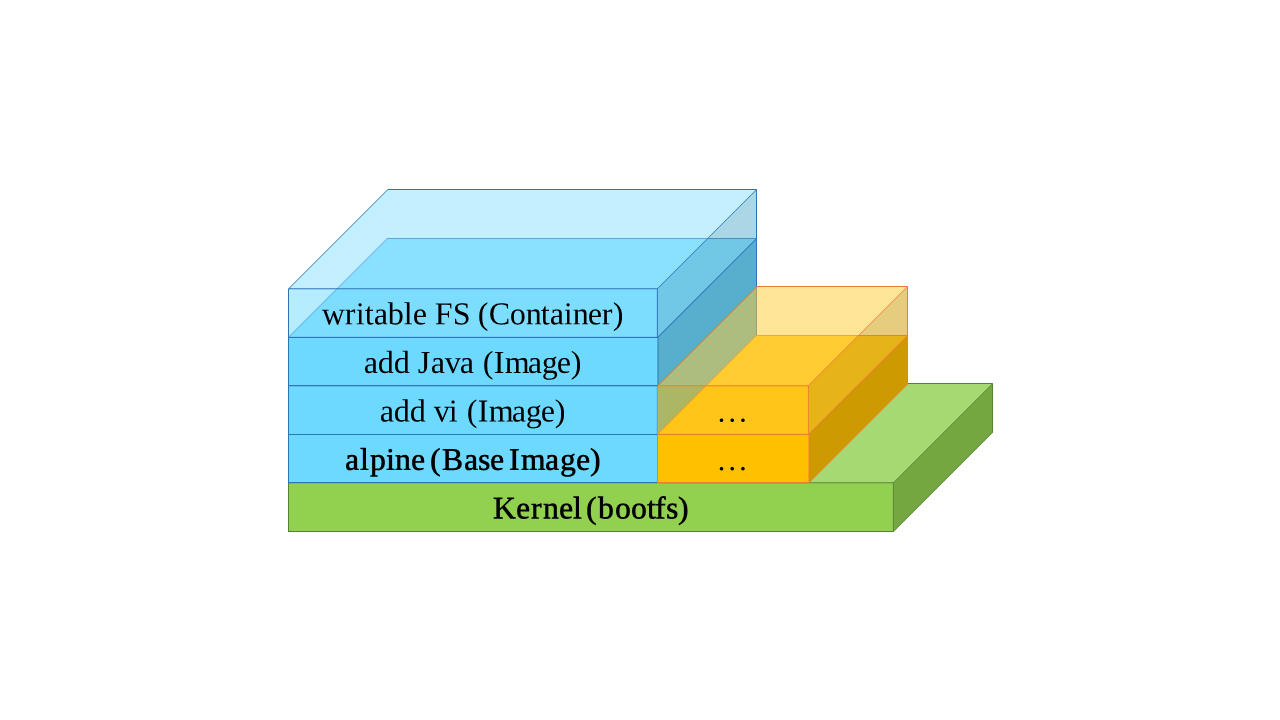
\includegraphics[width=0.7\linewidth,clip,trim=130 130 130 110]{images/docker-filesystem}
    \caption{Docker-Dateisystem}
\label{fig:docker-dateisystem}
\end{figure}
Jedes Image besteht aus mehreren gestapelten Schichten.
Die einzelnen Schichten merken dies allerdings nicht.
Jede dieser Schichten bekommt eine kombinierte Sicht auf alle darunterliegenden.
Sie kann selbst Dateien hinzufügen, ändern oder als gelöscht markieren, ändert allerdings die darunterliegenden Schichten nicht.
Diese Idee eines Dateisystems wird Union File System genannt.

Genau dadurch wird Docker sehr speichereffizient, da idente Schichten nur einmal existieren.
Ein Image, das auf einem anderen aufbaut, teilt sich dieselbe Basisschicht, welche durch einen eindeutigen Hash identifiziert, wiederverwendet werden kann.
Dadurch wird auch beim Start von zahlreichen identen Containern beinahe kein Speicherplatz benötigt, denn die schreibgeschützte Image-Schicht ist bei jedem Container ident.


\section{Dockerfiles}
\label{sec:dockerfiles}
\subsubsection{Reduktion der Imagegröße}
\subsubsection{CMD vs. ENTRYPOINT}

% - Layers
% - ...
% - http://bitjudo.com/blog/2014/03/13/building-efficient-dockerfiles-node-dot-js/
% - Example: https://nodejs.org/en/docs/guides/nodejs-docker-webapp/ (http://jdlm.info/articles/2016/03/06/lessons-building-node-app-docker.html)
% - https://www.brandpending.com/2016/06/14/building-nodejs-with-npm-dependencies-into-a-docker-container-without-using-a-dockerfile/ ???
% - Faster Builds: http://thenewstack.io/understanding-the-docker-cache-for-faster-builds/
% - Building good Images
% - https://blog.replicated.com/2016/02/05/refactoring-a-dockerfile-for-image-size/
% - https://nickjanetakis.com/blog/alpine-based-docker-images-make-a-difference-in-real-world-apps
% - http://blog.xebia.com/create-the-smallest-possible-docker-container/

% - ENTRYPOINT vs. CMD
% - https://www.ctl.io/developers/blog/post/dockerfile-entrypoint-vs-cmd/
% - http://goinbigdata.com/docker-run-vs-cmd-vs-entrypoint/
% - http://www.projectatomic.io/docs/docker-image-author-guidance/
% \section{Multi-Container-Anwendungen} % - Namen überdenken!!!
% \label{sec:docker-multi-container-anwendungen}
% - fig vs. docker-compose
% - Bash-Skripte vs. docker-compose
% - bei größeren Systemen auf Kapitel 1 (Orchestration) verweisen
% - https://ypereirareis.github.io/blog/2015/05/04/docker-with-shell-script-or-makefile/
% - http://codereview.stackexchange.com/questions/137877/shell-script-wrapper-for-docker-build-and-run
% - https://github.com/JonathonReinhart/scuba -> Simple Container-Utilizing Build Apparatus
% - https://blog.codeship.com/cross-platform-docker-development-environment/
% - stack
%  - https://docs.docker.com/docker-cloud/apps/stacks/
%  - https://blog.nimbleci.com/2016/09/14/docker-stacks-and-why-we-need-them/
%  - https://blog.couchbase.com/2016/july/docker-services-stack-distributed-application-bundle
\section{Häufig benötigte Docker-Kommandos}
\label{docker-kommandos}
% - http://jimhoskins.com/2013/07/27/remove-untagged-docker-images.html
% - Scripting
% - https://rominirani.com/docker-management-commands-e89a23c55908#.wlq1ixs5i

% docker build
% docker run --rm -it -v
% docker rmi (cleanup)
% new docker command line
